\documentclass[a4paper,10pt]{article}
\usepackage{longtable}
\usepackage[utf8]{inputenc}
\usepackage{url}
\usepackage{hyperref}
\usepackage{listings}
\usepackage{color}
\usepackage{verbatim}
\definecolor{grey}{rgb}{0.9,0.9,0.9}
\usepackage{float}
\usepackage{graphicx}
\usepackage{fancyhdr}
%\pagestyle{fancy} % voir si laisse ce style ou pas ?
%\usepackage[top=2.5cm,bottom=2.5cm,right=2.5cm,left=2.5cm]{geometry}
\usepackage[right=4cm,left=4cm]{geometry}
\lstset{
language=C++,
basicstyle=\footnotesize\fontfamily{pcr},
backgroundcolor=\color{grey},
numbers=left,
numberstyle=\tiny,
numbersep=5pt,
showstringspaces=false,
tabsize=2,
breaklines=true
}


% Title Page
\title{INFO-F403 Introduction to Language Theory and Compilation}
\author{Chapeaux Thomas\\Dagnely Pierre}

\begin{document}
\maketitle


\pagebreak
%%%%%%%%%%%%%%%%%%%%%%%%%%%%%%%%%%%%%%%%%%%%%%%%%%%%%%%%%%%%%%%%%%%%%%%%%%%%%%%%%%%%%%%%%%%%%%%%%%%%%%%%%%%%%%%%%%%%%%%%%%%%%%%%%%%%%%%%%
%%
%%
%%	Quenstion 1
%%
%%
%%%%%%%%%%%%%%%%%%%%%%%%%%%%%%%%%%%%%%%%%%%%%%%%%%%%%%%%%%%%%%%%%%%%%%%%%%%%%%%%%%%%%%%%%%%%%%%%%%%%%%%%%%%%%%%%%%%%%%%%%%%%%%%%%%%%%%%%%%

\section{Lexèmes}

Définition des tokens~\\

\begin{tabular}{cc}

\begin{tabular}{|c|l|}
\hline
Lexical units  		& regular expressions \\ \hline
INT					& ([0-9])* \\ \hline
FLOAT				& ([0-9])*.DOT.([0-9])* \\ \hline
BOOL				& (0+1+true+false+'') \\ \hline
STRING				& '.([A-Za-z]+[0-9])*.'  \\ \hline
FAC					& ! \\ \hline
MUL					& * \\ \hline
DIV					& / \\ \hline
MINUS				& - \\ \hline
ADD					& + \\ \hline
LT					& $<$ \\ \hline
GT					& $>$ \\ \hline
LE					& $<=$ \\ \hline
GE					& $>=$ \\ \hline
EQUIV				& == \\ \hline
DIF					& != \\ \hline
AND					& \&\& \\ \hline
OR					& $||$ \\ \hline
NOT					& not \\ \hline
LT-S				& lt \\ \hline
GT-S				& gt \\ \hline
LE-S				& le \\ \hline
GE-S				& ge \\ \hline
EQ-S				& eq \\ \hline 
NE-S				& ne \\ \hline
\end{tabular}

&

\begin{tabular}{|c|l|}
\hline
Lexical units  		& regular expressions \\ \hline
EQUAL				& = \\ \hline
DOT					& . \\ \hline
SEMICOLON			& ; \\ \hline
COMA				& , \\ \hline
OPEN-PAR			& ( \\ \hline
CLOSE-PAR			& ) \\ \hline
OPEN-BRAC			& \{ \\ \hline
CLOSE-BRAC			& \} \\ \hline
OPEN-COND			& IF \\ \hline
CLOSE-COND 			& ELSE \\ \hline
ADD-COND			& ELSE IF \\ \hline
NEG-COND			& UNLESS \\ \hline
RET					& return \\ \hline
FUNCT-DEF			& SUB \\ \hline
ID					& STRING \\ \hline 
FUNCT-CALL			& \&.STRING \\ \hline
PERL-DEF			& defined  \\ \hline
PERL-INT			& int  \\ \hline
PERL-LENG			& length  \\ \hline
PERL-SCAL			& scalar  \\ \hline
PERL-SUBS			& substr  \\ \hline
PERL-PRIN			& print\\ \hline
COMM				& \#.STRING \\ \hline
VARIABLE			& \$.STRING \\ \hline
					


\end{tabular}
\end{tabular}
~\\

coma peut définir l'opérateur coma ou juste un coma entre deux param, mais même lexical unit, c'est le parser qui se charge du reste


\pagebreak
\section{Automates}

Définition des automates finis
~\\
\paragraph{DFA}~\\

 \begin{figure}[H] \hspace*{-2cm} 
    \centering
   	  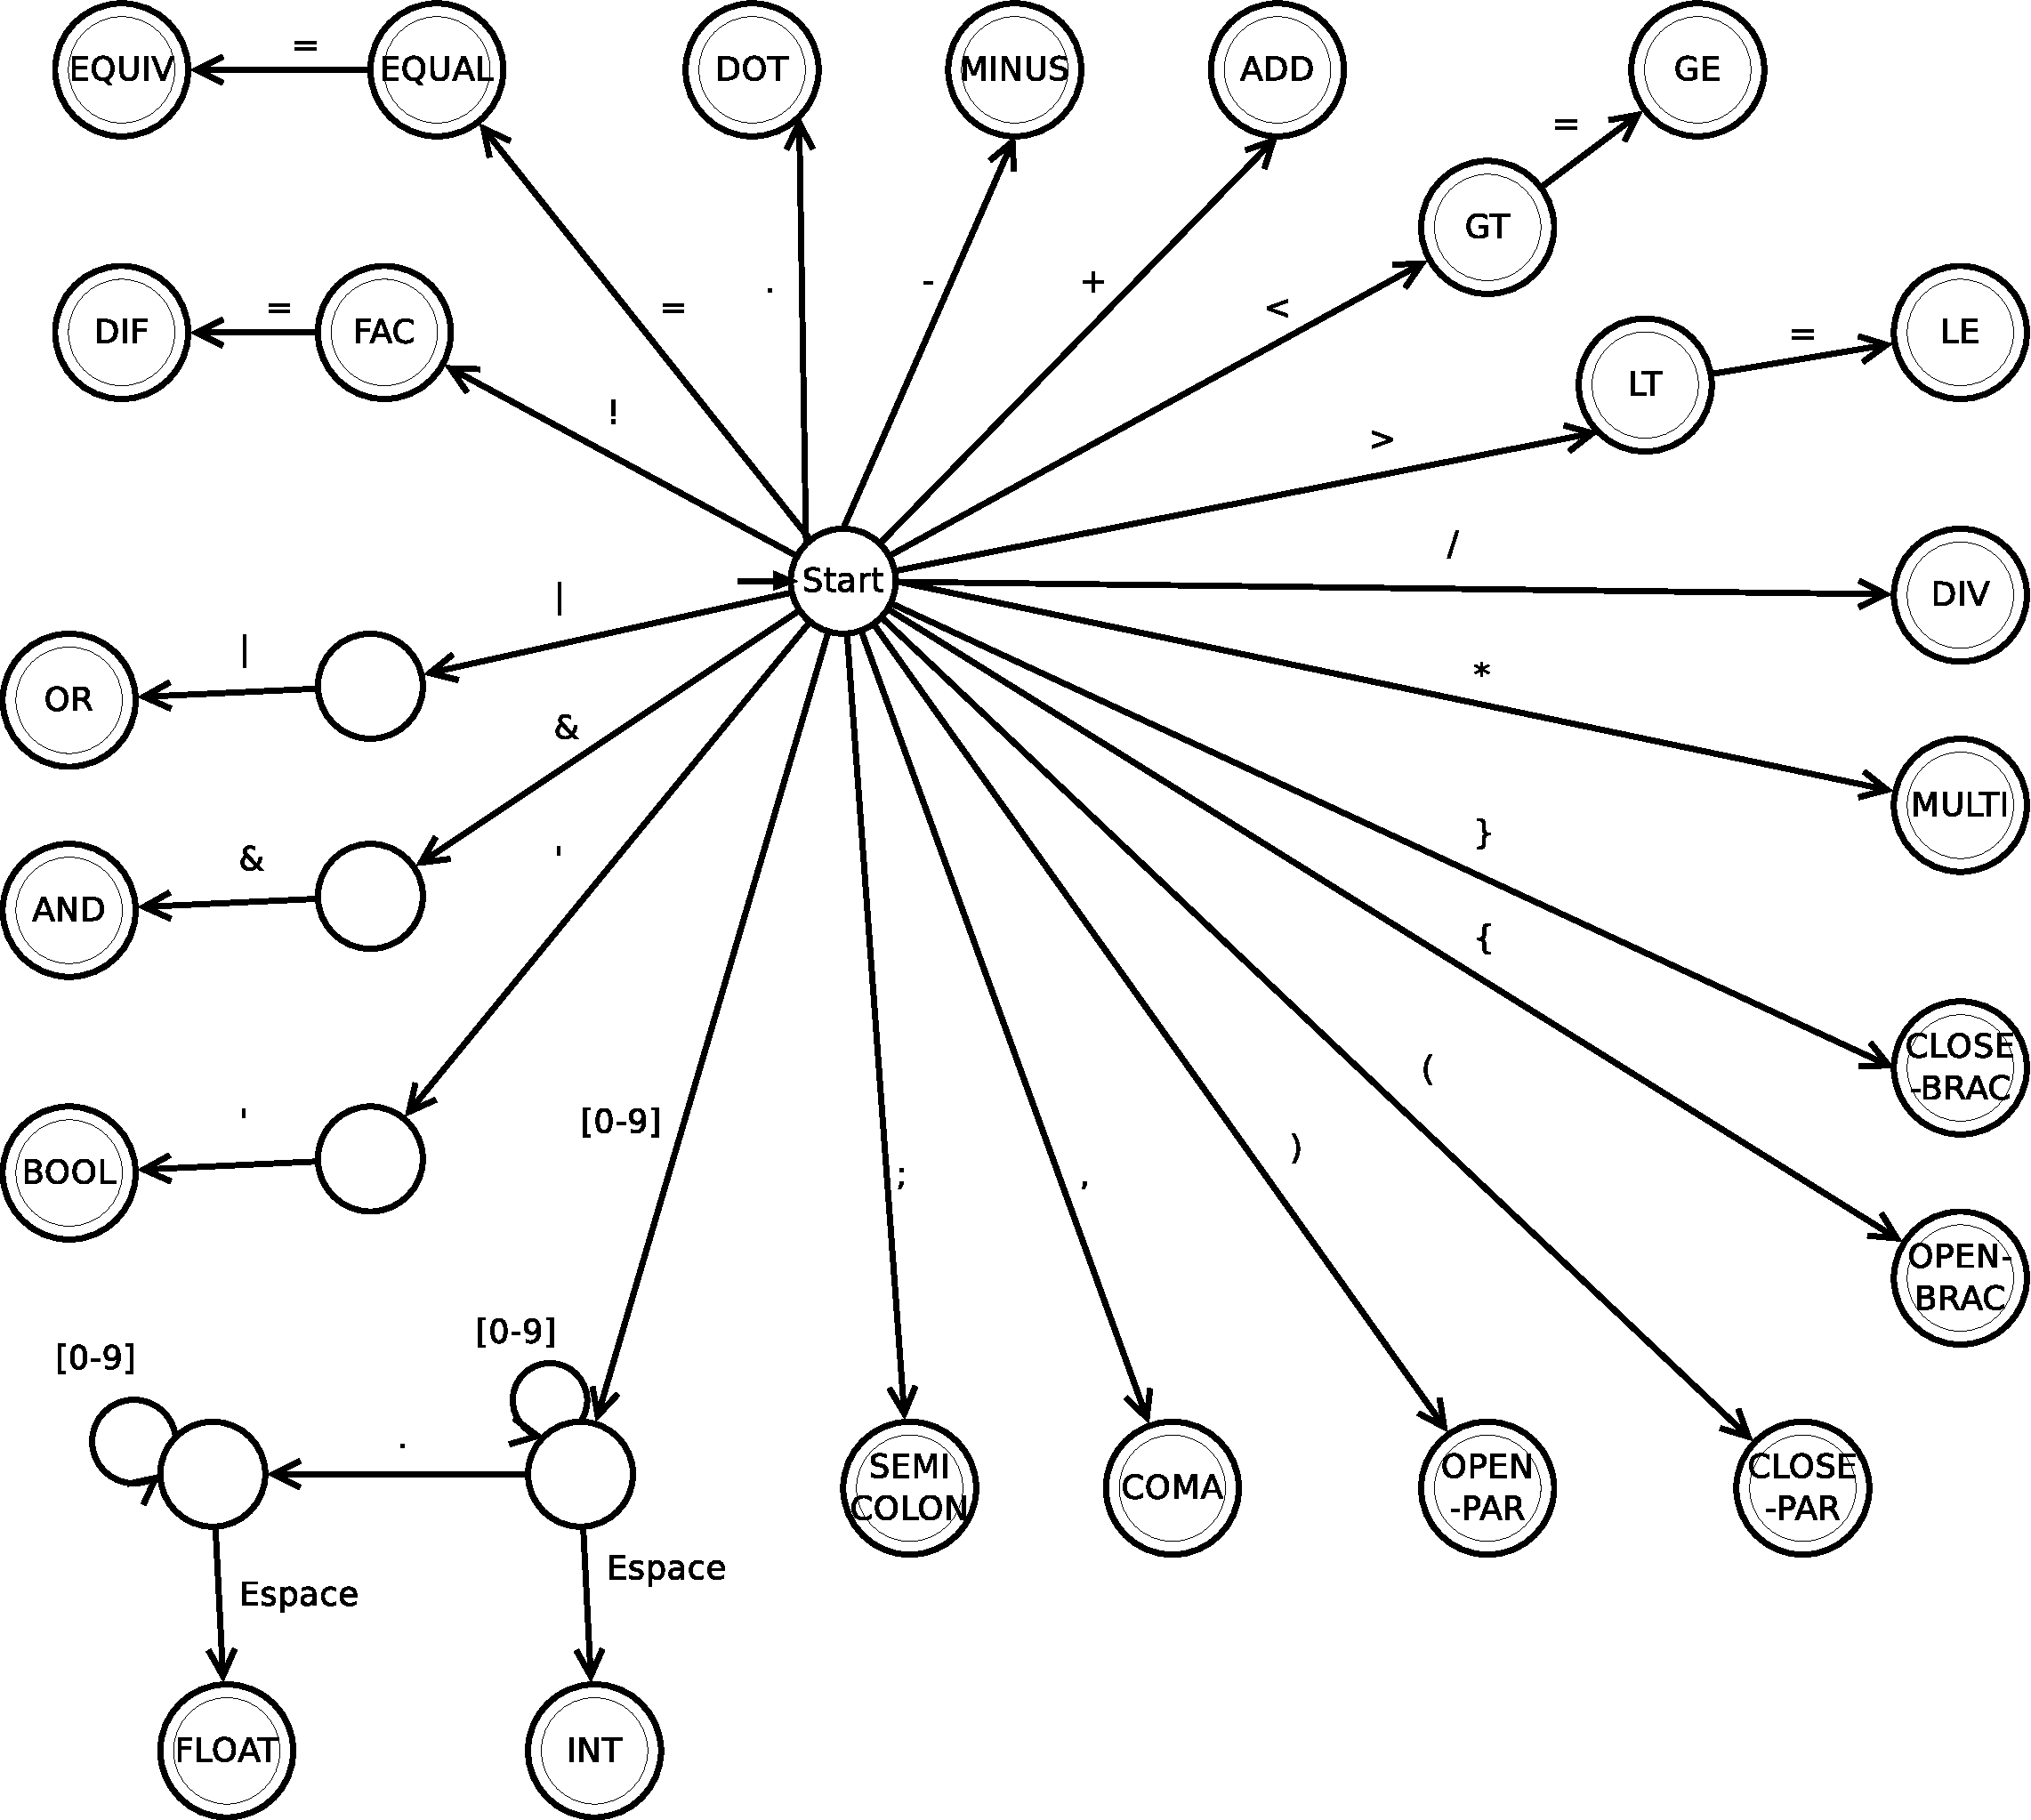
\includegraphics[width=400pt]{automate1.pdf} 
			\caption{automate "non alphabétique"}
			\label{automate1}
  \end{figure}	
  
	La plupart des noeuds pointent vers le token ID, trop lourd a représenter, donc met une petite fleche bleu à la place.  
  
  \begin{figure}[H] \hspace*{-2cm} 
    \centering
   	  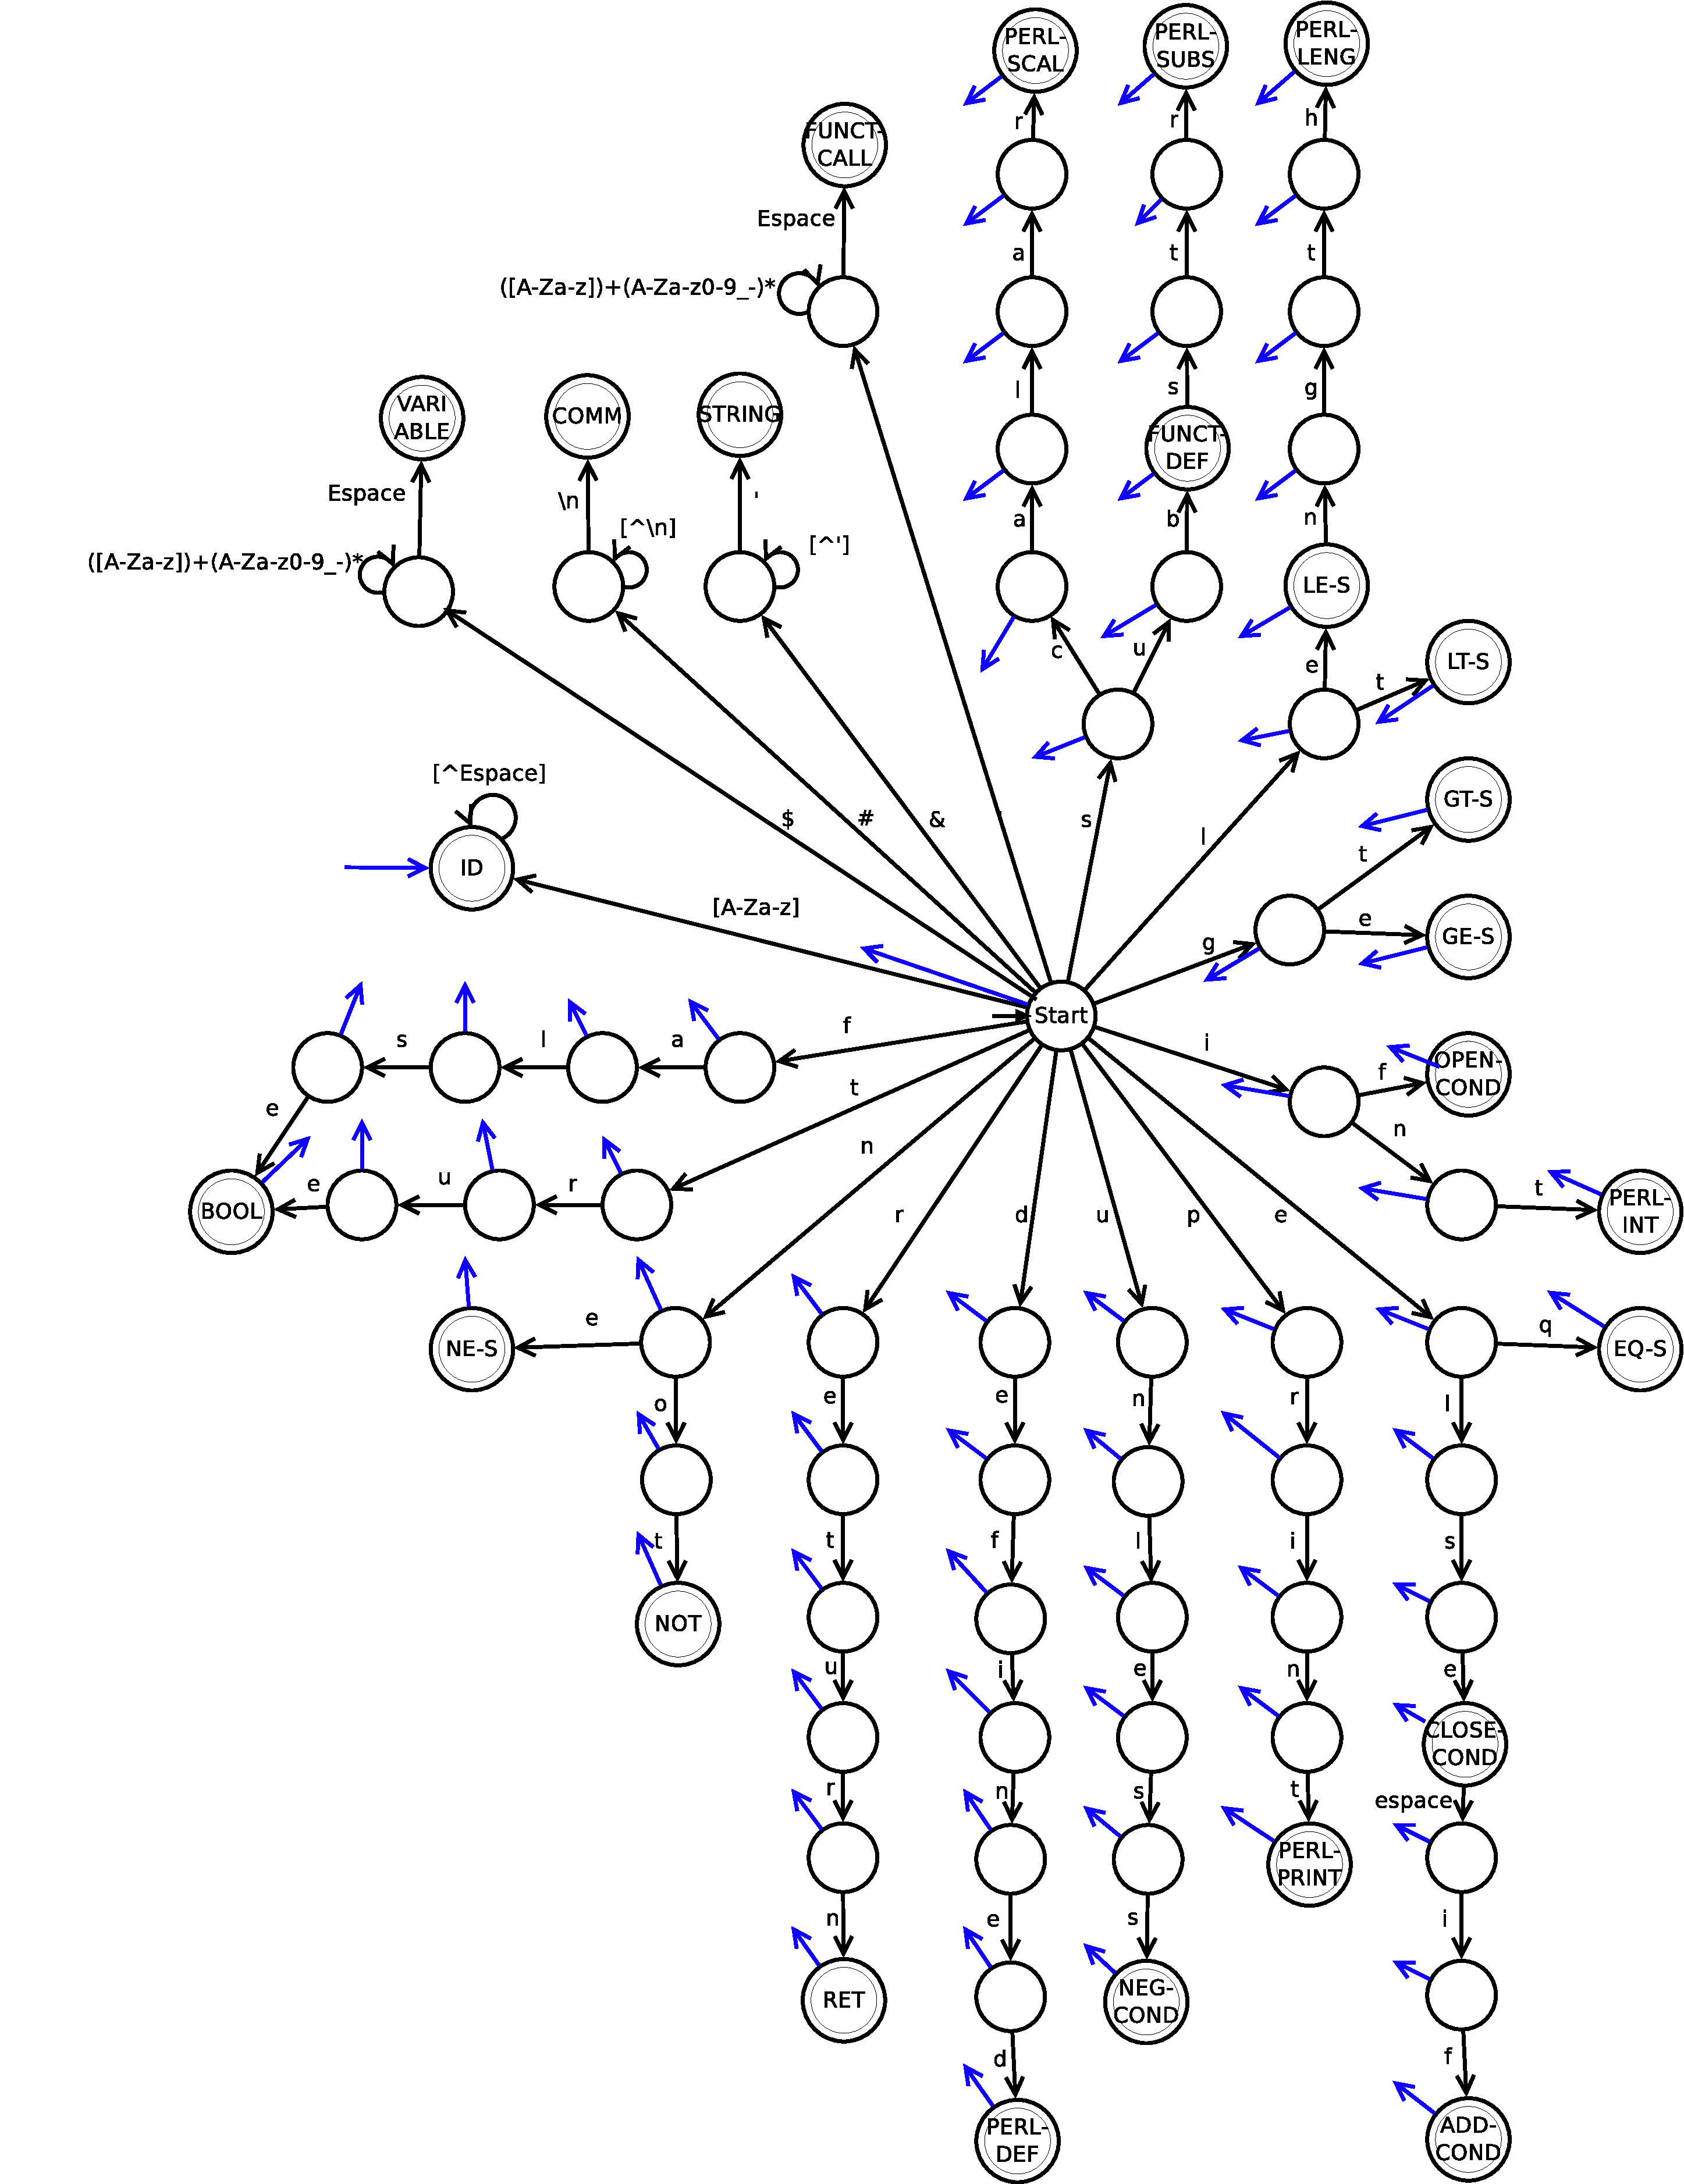
\includegraphics[width=450pt]{automate2.pdf} 
			\caption{automate "alphabétique"}
			\label{automate2}
  \end{figure}	

\pagebreak
~\\

\section{Gramaires}

\subsection{Définition de la grammaire}

On se base sur la BNF donné par l'assistant et on l'adapte à notre version de perl

\hspace{-4.5cm}\begin{tabular}{rl}
PROGRAM				& $\rightarrow$ PROGRAM FUNCT-LIST\\
					& $\rightarrow$ PROGRAM INSTRUCT\\
					& $\rightarrow$ FUNCT-LIST\\
					& $\rightarrow$ INSTRUCT\\
					& $\rightarrow$ EPSILON\\
					
					
FUNCT-LIST			& $\rightarrow$ FUNCT \\
					& $\rightarrow$ FUNCT FUNCT-LIST\\
					& $\rightarrow$ EPSILON\\
					
FUNCT				& $\rightarrow$ FUNCT-ID FUNCT-NAME OPEN-BRAC INSTRUCT RETURN CLOSE-BRAC \\
					& $\rightarrow$ FUNCT-ID FUNCT-NAME OPEN-PAR CLOSE PAR OPEN-BRAC INSTRUCT RETURN CLOSE-BRAC \\
					& $\rightarrow$ FUNCT-ID FUNCT-NAME OPEN-PAR PARAM CLOSE-PAR OPEN-BRAC INSTRUCT RETURN CLOSE-BRAC \\

FUNCT-CALL			& $\rightarrow$ USER-FUNCT-CALL \\
					& $\rightarrow$ PERL-FUNCT-CALL \\

USER-FUNCT-CALL		& $\rightarrow$ FUNCT-NAME OPEN-PAR CLOSE-PAR\\ 
					& $\rightarrow$ FUNCT-NAME OPEN-PAR PARAM CLOSE-PAR\\ 
					& $\rightarrow$ FUNCT-NAME PARAM\\ 
					& $\rightarrow$ FUNCT-NAME\\ 

				
PERL-FUNCT-CALL		& $\rightarrow$ PERL-DEF EXP \\
					& $\rightarrow$ PERL-INT EXP \\
					& $\rightarrow$ PERL-LENG EXP \\ 
					& $\rightarrow$ PERL-SCAL EXP \\
					& $\rightarrow$ PERL-SUBS EXP COMA INT COMA INT \\
					& $\rightarrow$ PERL-SUBS EXP COMA INT  \\
					& $\rightarrow$ PERL-PRIN LIST \\ 
					
LIST				& $\rightarrow$ STRING \\
					& $\rightarrow$ STRING LIST\\
					& $\rightarrow$ EPSILON\\
				

					
PARAM				& $\rightarrow$ VAR \\
					& $\rightarrow$ VAR PARAM-END\\
					& $\rightarrow$ EPSILON \\
PARAM-END			& $\rightarrow$ COMA VAR \\ 
					& $\rightarrow$ COMA VAR PARAM-END\\ 
					& $\rightarrow$ EPSILON \\

RETURN				& $\rightarrow$ RET EXP SEMICOLON\\
					& $\rightarrow$ RET EXP-COND SEMICOLON\\
					& $\rightarrow$ RET VAR SEMICOLON\\
					& $\rightarrow$ EPSILON \\
					



					
					
\end{tabular}

~\\

\hspace{-4.5cm}\begin{tabular}{rl}


INSTRUCT			& $\rightarrow$ COND SEMICOLON INSTRUCT\\
					& $\rightarrow$ EXP SEMICOLON INSTRUCT\\
					& $\rightarrow$ FUNCT-CALL SEMICOLON INSTRUCT\\
					& $\rightarrow$ ASSIGNATION SEMICOLON INSTRUCT\\
					& $\rightarrow$ COND SEMICOLON \\
					& $\rightarrow$ EXP SEMICOLON \\
					& $\rightarrow$ FUNCT-CALL SEMICOLON \\
					& $\rightarrow$ ASSIGNATION SEMICOLON \\
					& $\rightarrow$ EPSILON \\
					

ASSIGNATION			& $\rightarrow$ VAR EQUAL VALUE \\
					& $\rightarrow$ VAR EQUAL EXP \\
					
COND				& $\rightarrow$ OPEN-COND EXP-COND OPEN-BRAC INSTRUCT CLOSE-BRAC COND-END\\
					& $\rightarrow$ NEG-COND EXP-COND OPEN-BRAC INSTRUCT CLOSE-BRAC COND-END\\
					& $\rightarrow$ EXP OPEN-COND EXP-COND \\
					& $\rightarrow$ EXP NEG-COND EXP-COND \\


COND-END			& $\rightarrow$ ADD-COND EXP-COND OPEN-BRAC INSTRUCT CLOSE-BRAC \\
					& $\rightarrow$ ADD-COND EXP-COND OPEN-BRAC INSTRUCT CLOSE-BRAC COND-END \\
					& $\rightarrow$ CLOSE-COND OPEN-BRAC INSTRUCT CLOSE-BRAC\\
					& $\rightarrow$ EPSILON \\					

EXP					& $\rightarrow$ VAR   \\
					& $\rightarrow$ EXP OPERATOR EXP \\ 
					& $\rightarrow$ EXP-COMP \\
					& $\rightarrow$ NOT EXP \\
					& $\rightarrow$ FAC EXP \\
					& $\rightarrow$ ADD EXP \\
					& $\rightarrow$ MINUS EXP \\
					
EXP-COMP			& $\rightarrow$ EXP OPERATOR-COMP EXP \\

OPERATOR			& $\rightarrow$ MUL \\ 
					& $\rightarrow$ DIV \\ 
					& $\rightarrow$ MINUS \\ 
					& $\rightarrow$ CONC \\ 
					& $\rightarrow$ ADD	\\ 
OPERATOR-COMP		& $\rightarrow$ LT\\
					& $\rightarrow$ GT	\\
					& $\rightarrow$ LE	\\
					& $\rightarrow$ GE	\\
					& $\rightarrow$ EQUIV	\\
					& $\rightarrow$ DIF	\\
					& $\rightarrow$ AND-LOGIC	\\
					& $\rightarrow$ OR		\\
					& $\rightarrow$ LT-S\\
					& $\rightarrow$ GT-S\\
					& $\rightarrow$ LE-S	\\
					& $\rightarrow$ GE-S	\\
					& $\rightarrow$ COMA-LOGIC	\\
					& $\rightarrow$ EQ-S	\\
					& $\rightarrow$ NE-S	\\

VALUE				& $\rightarrow$ INT \\
					& $\rightarrow$ FLOAT \\
					& $\rightarrow$ BOOL \\
					& $\rightarrow$ STRING \\
					
VAR					& $\rightarrow$ VALUE \\
					& $\rightarrow$ MINUS VAR\\
					& $\rightarrow$ ADD VAR \\
					& $\rightarrow$ OPEN-PAR EXP CLOSE-PAR \\

\end{tabular}

~\\

\subsection{Gestion des priorités}

On doit adapter la grammaire pour respecter les priorité et les associativité gauche/droite.\\
Cela ne modifie que les règles EXP, EXP-COND, OPERATOR et OPERATOR-COND qui deviennent : \\
~\\



\begin{tabular}{rl}


$<$EXP$>$			& $\rightarrow$ $<$EXP$>$ LT $<$EXP2$>$\\
					& $\rightarrow$ $<$EXP$>$ LT-S $<$EXP2$>$\\
					& $\rightarrow$ $<$EXP$>$ GT $<$EXP2$>$\\
					& $\rightarrow$ $<$EXP$>$ LT-S $<$EXP2$>$\\
					& $\rightarrow$ $<$EXP$>$ LE $<$EXP2$>$\\
					& $\rightarrow$ $<$EXP$>$ LE-S $<$EXP2$>$\\
					& $\rightarrow$ $<$EXP$>$ GE $<$EXP2$>$\\
					& $\rightarrow$ $<$EXP$>$ GE-S $<$EXP2$>$\\
					& $\rightarrow$ $<$EXP$>$ EQUIV $<$EXP2$>$\\
					& $\rightarrow$ $<$EXP$>$ DIF $<$EXP2$>$\\
					& $\rightarrow$ $<$EXP2$>$ EQUAL $<$EXP$>$\\
					& $\rightarrow$ NOT $<$EXP$>$ \\
					& $\rightarrow$ FAC $<$EXP$>$ \\
					& $\rightarrow$ $<$EXP2$>$ \\
										
					
$<$EXP2$>$			& $\rightarrow$ $<$EXP$>$ ADD $<$EXP3$>$\\
					& $\rightarrow$ $<$EXP$>$ MINUS $<$EXP3$>$\\
					& $\rightarrow$ $<$EXP$>$ OR $<$EXP3$>$\\
					& $\rightarrow$ $<$EXP3$>$\\
					
$<$EXP3$>$			& $\rightarrow$ $<$EXP$>$ MUL $<$VAR$>$\\
					& $\rightarrow$ $<$EXP$>$ DIV $<$VAR$>$\\
					& $\rightarrow$ $<$EXP$>$ AND $<$VAR$>$\\
					& $\rightarrow$ $<$VAR$>$\\
\end{tabular}





\subsection{Suppression des symboles inutiles}
On doit virer non-productifs et inaccessibles.\\
Ici ok, rien à faire







\subsection{left-factoring}
On vire ce qui commence pareillement~\\

On obtient la gram suivante : 

\hspace{-3.5cm}\begin{tabular}{rl}
PROGRAM				& $\rightarrow$ PROGRAM PROG-END \\
					& $\rightarrow$ FUNCT-LIST\\
					& $\rightarrow$ INSTRUCT\\
					& $\rightarrow$ EPSILON\\
PROG-END			& $\rightarrow$ FUNCT-LIST\\
					& $\rightarrow$ INSTRUCT\\
					
FUNCT-LIST			& $\rightarrow$ FUNCT FUNCT-LIST-END\\
					& $\rightarrow$ EPSILON\\
					
FUNCT-LIST-END		& $\rightarrow$ FUNCT-LIST\\
					& $\rightarrow$ EPSILON\\
					
FUNCT				& $\rightarrow$ FUNCT-ID FUNCT-NAME FUNCT-END \\

FUNCT-END			& $\rightarrow$ OPEN-BRAC INSTRUCT RETURN CLOSE-BRAC \\
					& $\rightarrow$ OPEN-PAR FUNCT-END2 \\

FUNCT-END2			& $\rightarrow$ CLOSE PAR OPEN-BRAC INSTRUCT RETURN CLOSE-BRAC \\
					& $\rightarrow$ PARAM CLOSE-PAR OPEN-BRAC INSTRUCT RETURN CLOSE-BRAC \\

FUNCT-CALL			& $\rightarrow$ USER-FUNCT-CALL \\
					& $\rightarrow$ PERL-FUNCT-CALL \\

USER-FUNCT-CALL		& $\rightarrow$ FUNCT-NAME USER-FUNCT-CALL-END\\ 

USER-FUNCT-CALL-END	& $\rightarrow$ OPEN-PAR USER-FUNCT-CALL-END2\\ 
					& $\rightarrow$ PARAM\\ 
					& $\rightarrow$ EPSILON\\
					
USER-FUNCT-CALL-END2& $\rightarrow$ CLOSE-PAR\\ 
					& $\rightarrow$ PARAM CLOSE-PAR\\ 

				
PERL-FUNCT-CALL		& $\rightarrow$ PERL-DEF EXP \\
					& $\rightarrow$ PERL-INT EXP \\
					& $\rightarrow$ PERL-LENG EXP \\ 
					& $\rightarrow$ PERL-SCAL EXP \\
					& $\rightarrow$ PERL-SUBS PERL-SUBS-END \\
					& $\rightarrow$ PERL-PRIN LIST \\ 
					
PERL-SUBS-END		& $\rightarrow$ EXP COMA INT COMA INT \\
					& $\rightarrow$ EXP COMA INT  \\
					
LIST				& $\rightarrow$ STRING LIST-END\\
					
LIST-END			& $\rightarrow$ LIST\\
					& $\rightarrow$ EPSILON\\
				

					
PARAM				& $\rightarrow$ PARAM2\\
					& $\rightarrow$ EPSILON \\

PARAM2				& $\rightarrow$ PARAM-END\\
					& $\rightarrow$ EPSILON \\
					
					
PARAM-END			& $\rightarrow$ COMA VAR PARAM-END2\\ 
					& $\rightarrow$ EPSILON \\
					
PARAM-END2			& $\rightarrow$ PARAM-END\\ 
					& $\rightarrow$ EPSILON \\

RETURN				& $\rightarrow$ RET RETURN-END\\
					& $\rightarrow$ EPSILON \\

RETURN-END			& $\rightarrow$ EXP SEMICOLON\\
					& $\rightarrow$ EXP-COND SEMICOLON\\
					& $\rightarrow$ VAR SEMICOLON\\

					
					
					



					
					
\end{tabular}

~\\

\hspace{-3.5cm}\begin{tabular}{rl}


INSTRUCT			& $\rightarrow$ COND INSTRUCT-END \\					
					& $\rightarrow$ EXP INSTRUCT-END \\					
					& $\rightarrow$ FUNCT-CALL INSTRUCT-END \\					
					& $\rightarrow$ ASSIGNATION INSTRUCT-END \\
					& $\rightarrow$ EPSILON \\

INSTRUCT-END		& $\rightarrow$ SEMICOLON INSTRUCT-END2\\

INSTRUCT-END2		& $\rightarrow$ INSTRUCT\\
					& $\rightarrow$ EPSILON \\
					

ASSIGNATION			& $\rightarrow$ VAR EQUAL ASSIGNATION-END \\

ASSIGNATION-END		& $\rightarrow$ VALUE \\
					& $\rightarrow$ EXP \\
					
COND				& $\rightarrow$ OPEN-COND EXP-COND OPEN-BRAC INSTRUCT CLOSE-BRAC COND-END\\
					& $\rightarrow$ NEG-COND EXP-COND OPEN-BRAC INSTRUCT CLOSE-BRAC COND-END\\
					& $\rightarrow$ EXP COND-END2 \\

COND-END2			& $\rightarrow$ OPEN-COND EXP-COND \\
					& $\rightarrow$ NEG-COND EXP-COND \\


COND-END			& $\rightarrow$ ADD-COND EXP-COND OPEN-BRAC INSTRUCT CLOSE-BRAC COND-END3 \\
					& $\rightarrow$ CLOSE-COND OPEN-BRAC INSTRUCT CLOSE-BRAC\\
					& $\rightarrow$ EPSILON \\	
					
COND-END3			& $\rightarrow$ COND-END \\
					& $\rightarrow$ EPSILON \\					

$<$EXP$>$			& $\rightarrow$ $<$EXP$>$ $<$EXP-END$>$\\
					& $\rightarrow$ $<$EXP2$>$ EQUAL $<$EXP$>$\\
					& $\rightarrow$ NOT $<$EXP$>$ \\
					& $\rightarrow$ FAC $<$EXP$>$ \\
					& $\rightarrow$ $<$EXP2$>$ \\
					
					
$<$EXP-END$>$		& $\rightarrow$ LT $<$EXP2$>$\\
					& $\rightarrow$ LT-S $<$EXP2$>$\\
					& $\rightarrow$ GT $<$EXP2$>$\\
					& $\rightarrow$ LT-S $<$EXP2$>$\\
					& $\rightarrow$ LE $<$EXP2$>$\\
					& $\rightarrow$ LE-S $<$EXP2$>$\\
					& $\rightarrow$ GE $<$EXP2$>$\\
					& $\rightarrow$ GE-S $<$EXP2$>$\\
					& $\rightarrow$ EQUIV $<$EXP2$>$\\
					& $\rightarrow$ DIF $<$EXP2$>$\\
										
					
$<$EXP2$>$			& $\rightarrow$ $<$EXP$>$ $<$EXP2-END$>$\\
					& $\rightarrow$ $<$EXP3$>$\\
					
$<$EXP2-END$>$		& $\rightarrow$  ADD $<$EXP3$>$\\
					& $\rightarrow$  MINUS $<$EXP3$>$\\
					& $\rightarrow$  OR $<$EXP3$>$\\					

					
$<$EXP3$>$			& $\rightarrow$ $<$EXP$>$ $<$EXP3-END$>$\\
					& $\rightarrow$ $<$VAR$>$\\
					
$<$EXP3-END$>$		& $\rightarrow$ MUL $<$VAR$>$\\
					& $\rightarrow$ DIV $<$VAR$>$\\
					& $\rightarrow$ AND $<$VAR$>$\\

VALUE				& $\rightarrow$ INT \\
					& $\rightarrow$ FLOAT \\
					& $\rightarrow$ BOOL \\
					& $\rightarrow$ STRING \\
					
VAR					& $\rightarrow$ VALUE \\
					& $\rightarrow$ MINUS VAR\\
					& $\rightarrow$ ADD VAR \\
					& $\rightarrow$ OPEN-PAR EXP CLOSE-PAR \\

\end{tabular}







\subsection{récursion gauche}




\pagebreak
\subsection{Grammaire finale}
\textbf{VERSION PROVISOIRE !!!!!!!!!!!!!!!!!!!!!!!!!!!}
~\\
\hspace{-3.5cm}\begin{tabular}{rl}
PROGRAM				& $\rightarrow$ PROGRAM PROG-END \\
					& $\rightarrow$ FUNCT-LIST\\
					& $\rightarrow$ INSTRUCT\\
					& $\rightarrow$ EPSILON\\
PROG-END			& $\rightarrow$ FUNCT-LIST\\
					& $\rightarrow$ INSTRUCT\\
					
FUNCT-LIST			& $\rightarrow$ FUNCT FUNCT-LIST-END\\
					& $\rightarrow$ EPSILON\\
					
FUNCT-LIST-END		& $\rightarrow$ FUNCT-LIST\\
					& $\rightarrow$ EPSILON\\
					
FUNCT				& $\rightarrow$ FUNCT-ID FUNCT-NAME FUNCT-END \\

FUNCT-END			& $\rightarrow$ OPEN-BRAC INSTRUCT RETURN CLOSE-BRAC \\
					& $\rightarrow$ OPEN-PAR FUNCT-END2 \\

FUNCT-END2			& $\rightarrow$ CLOSE PAR OPEN-BRAC INSTRUCT RETURN CLOSE-BRAC \\
					& $\rightarrow$ PARAM CLOSE-PAR OPEN-BRAC INSTRUCT RETURN CLOSE-BRAC \\

FUNCT-CALL			& $\rightarrow$ USER-FUNCT-CALL \\
					& $\rightarrow$ PERL-FUNCT-CALL \\

USER-FUNCT-CALL		& $\rightarrow$ FUNCT-NAME USER-FUNCT-CALL-END\\ 

USER-FUNCT-CALL-END	& $\rightarrow$ OPEN-PAR USER-FUNCT-CALL-END2\\ 
					& $\rightarrow$ PARAM\\ 
					& $\rightarrow$ EPSILON\\
					
USER-FUNCT-CALL-END2& $\rightarrow$ CLOSE-PAR\\ 
					& $\rightarrow$ PARAM CLOSE-PAR\\ 

				
PERL-FUNCT-CALL		& $\rightarrow$ PERL-DEF EXP \\
					& $\rightarrow$ PERL-INT EXP \\
					& $\rightarrow$ PERL-LENG EXP \\ 
					& $\rightarrow$ PERL-SCAL EXP \\
					& $\rightarrow$ PERL-SUBS PERL-SUBS-END \\
					& $\rightarrow$ PERL-PRIN LIST \\ 
					
PERL-SUBS-END		& $\rightarrow$ EXP COMA INT COMA INT \\
					& $\rightarrow$ EXP COMA INT  \\
					
LIST				& $\rightarrow$ STRING LIST-END\\
					
LIST-END			& $\rightarrow$ LIST\\
					& $\rightarrow$ EPSILON\\
				

					
PARAM				& $\rightarrow$ PARAM2\\
					& $\rightarrow$ EPSILON \\

PARAM2				& $\rightarrow$ PARAM-END\\
					& $\rightarrow$ EPSILON \\
					
					
PARAM-END			& $\rightarrow$ COMA VAR PARAM-END2\\ 
					& $\rightarrow$ EPSILON \\
					
PARAM-END2			& $\rightarrow$ PARAM-END\\ 
					& $\rightarrow$ EPSILON \\

RETURN				& $\rightarrow$ RET RETURN-END\\
					& $\rightarrow$ EPSILON \\

RETURN-END			& $\rightarrow$ EXP SEMICOLON\\
					& $\rightarrow$ EXP-COND SEMICOLON\\
					& $\rightarrow$ VAR SEMICOLON\\
					
\end{tabular}


\hspace{-3.5cm}\begin{tabular}{rl}
INSTRUCT			& $\rightarrow$ COND INSTRUCT-END \\					
					& $\rightarrow$ EXP INSTRUCT-END \\					
					& $\rightarrow$ FUNCT-CALL INSTRUCT-END \\					
					& $\rightarrow$ ASSIGNATION INSTRUCT-END \\
					& $\rightarrow$ EPSILON \\

INSTRUCT-END		& $\rightarrow$ SEMICOLON INSTRUCT-END2\\

INSTRUCT-END2		& $\rightarrow$ INSTRUCT\\
					& $\rightarrow$ EPSILON \\
					

ASSIGNATION			& $\rightarrow$ VAR EQUAL ASSIGNATION-END \\

ASSIGNATION-END		& $\rightarrow$ VALUE \\
					& $\rightarrow$ EXP \\
					
COND				& $\rightarrow$ OPEN-COND EXP-COND OPEN-BRAC INSTRUCT CLOSE-BRAC COND-END\\
					& $\rightarrow$ NEG-COND EXP-COND OPEN-BRAC INSTRUCT CLOSE-BRAC COND-END\\
					& $\rightarrow$ EXP COND-END2 \\

COND-END2			& $\rightarrow$ OPEN-COND EXP-COND \\
					& $\rightarrow$ NEG-COND EXP-COND \\


COND-END			& $\rightarrow$ ADD-COND EXP-COND OPEN-BRAC INSTRUCT CLOSE-BRAC COND-END3 \\
					& $\rightarrow$ CLOSE-COND OPEN-BRAC INSTRUCT CLOSE-BRAC\\
					& $\rightarrow$ EPSILON \\	
					
COND-END3			& $\rightarrow$ COND-END \\
					& $\rightarrow$ EPSILON \\					

$<$EXP$>$			& $\rightarrow$ $<$EXP$>$ $<$EXP-END$>$\\
					& $\rightarrow$ $<$EXP2$>$ EQUAL $<$EXP$>$\\
					& $\rightarrow$ NOT $<$EXP$>$ \\
					& $\rightarrow$ FAC $<$EXP$>$ \\
					& $\rightarrow$ $<$EXP2$>$ \\
					
					
$<$EXP-END$>$		& $\rightarrow$ LT $<$EXP2$>$\\
					& $\rightarrow$ LT-S $<$EXP2$>$\\
					& $\rightarrow$ GT $<$EXP2$>$\\
					& $\rightarrow$ LT-S $<$EXP2$>$\\
					& $\rightarrow$ LE $<$EXP2$>$\\
					& $\rightarrow$ LE-S $<$EXP2$>$\\
					& $\rightarrow$ GE $<$EXP2$>$\\
					& $\rightarrow$ GE-S $<$EXP2$>$\\
					& $\rightarrow$ EQUIV $<$EXP2$>$\\
					& $\rightarrow$ DIF $<$EXP2$>$\\
										
					
$<$EXP2$>$			& $\rightarrow$ $<$EXP$>$ $<$EXP2-END$>$\\
					& $\rightarrow$ $<$EXP3$>$\\
					
$<$EXP2-END$>$		& $\rightarrow$  ADD $<$EXP3$>$\\
					& $\rightarrow$  MINUS $<$EXP3$>$\\
					& $\rightarrow$  OR $<$EXP3$>$\\					

					
$<$EXP3$>$			& $\rightarrow$ $<$EXP$>$ $<$EXP3-END$>$\\
					& $\rightarrow$ $<$VAR$>$\\
					
$<$EXP3-END$>$		& $\rightarrow$ MUL $<$VAR$>$\\
					& $\rightarrow$ DIV $<$VAR$>$\\
					& $\rightarrow$ AND $<$VAR$>$\\

VALUE				& $\rightarrow$ INT \\
					& $\rightarrow$ FLOAT \\
					& $\rightarrow$ BOOL \\
					& $\rightarrow$ STRING \\
					
VAR					& $\rightarrow$ VALUE \\
					& $\rightarrow$ MINUS VAR\\
					& $\rightarrow$ ADD VAR \\
					& $\rightarrow$ OPEN-PAR EXP CLOSE-PAR \\

\end{tabular}
~\\
















\section{Poubelle}





~\\
\pagebreak
\hspace{-4.5cm}\begin{tabular}{|c|l|}
\hline
EXPRESSION (?)		& VARIABLE OPERATOR VARIABLE   \\
					& EXPRESSION OPERATOR VARIABLE \\ \hline
EXPRESSION-COND (?)	& VARIABLE OPERATOR-COMP VARIABLE   \\
					& EXPRESSION OPERATOR-COMP VARIABLE \\ \hline
ASSIGNATION			& VARIABLE EQUAL VALUE \\ \hline
CONDITION (?)		& ((OPEN-COND+NEG-COND)EXPRESSION-COND OPEN-BRAC INSTRUCTIONS* CLOSE-BRAC\\
					& (ADD-COND EXPRESSION-COND OPEN-BRAC INSTRUCTIONS* CLOSE-BRAC)* \\
					& (CLOSE-COND EXPRESSION-COND OPEN-BRAC INSTRUCTIONS* CLOSE-BRAC))\\
					& + EXPRESSION (OPEN-COND + NEG-COND) EXPRESSION-COND \\ \hline
INSTRUCTIONS		& ((CONDITION SEMICOLON)* + (EXPRESSION SEMICOLON)* + (FUNCTION-CALL \\ 
					& SEMICOLON)* + (ASSIGNATION SEMICOLON)*)* \\ \hline
PARAM				& DOLLAR VARIABLE (COMA DOLLAR VARIABLE)* \\ \hline
USER-FUNCT-CALL		& AND FUNCTION-NAME (OPEN-PAR CLOSE-PAR + OPEN-PAR PARAM CLOSE-PAR  \\
					& + PARAM) SEMICOLON \\ \hline
PERL-FUNCT-CALL		& defined EXPRESSION + int EXPRESSION + length EXPRESSION \\ 
					& scalar EXPRESSION + substr EXPRESSION COMA INT COMA INT \\
					& scalar EXPRESSION + substr EXPRESSION COMA INT  \\
					& + print (?liste de string) \\ \hline
FUNCTION-CALL		& USER-FUNCT-CALL + PERL-FUNCT-CALL \\ \hline
FUNCTION			& FUNCTION-ID FUNCTION-NAME (OPEN-PAR CLOSE PAR + OPEN-PAR PARAM CLOSE-PAR) \\
					& OPEN-BRAC INSTRUCTIONS (RETURN EXPRESSION + RETURN EXPRESSION-COND \\
					& + RETURN VARIABLE) SEMICOLON CLOSE-BRAC \\ \hline
FUNCTION-LIST		& FUNCTION* \\ \hline
PROGRAM				& (FUNCTION-LIST + INSTRUCTIONS)*\\ \hline

					
					
\end{tabular}



~\\

Grammaire après gestion des priorité et associativité :

\hspace{-4.5cm}\begin{tabular}{rl}
PROGRAM				& $\rightarrow$ PROGRAM FUNCT-LIST\\
					& $\rightarrow$ PROGRAM INSTRUCT\\
					& $\rightarrow$ FUNCT-LIST\\
					& $\rightarrow$ INSTRUCT\\
					& $\rightarrow$ EPSILON\\
					
					
FUNCT-LIST			& $\rightarrow$ FUNCT \\
					& $\rightarrow$ FUNCT FUNCT-LIST\\
					& $\rightarrow$ EPSILON\\
					
FUNCT				& $\rightarrow$ FUNCT-ID FUNCT-NAME OPEN-BRAC INSTRUCT RETURN CLOSE-BRAC \\
					& $\rightarrow$ FUNCT-ID FUNCT-NAME OPEN-PAR CLOSE PAR OPEN-BRAC INSTRUCT RETURN CLOSE-BRAC \\
					& $\rightarrow$ FUNCT-ID FUNCT-NAME OPEN-PAR PARAM CLOSE-PAR OPEN-BRAC INSTRUCT RETURN CLOSE-BRAC \\

FUNCT-CALL			& $\rightarrow$ USER-FUNCT-CALL \\
					& $\rightarrow$ PERL-FUNCT-CALL \\

USER-FUNCT-CALL		& $\rightarrow$ FUNCT-NAME OPEN-PAR CLOSE-PAR\\ 
					& $\rightarrow$ FUNCT-NAME OPEN-PAR PARAM CLOSE-PAR\\ 
					& $\rightarrow$ FUNCT-NAME PARAM\\ 
					& $\rightarrow$ FUNCT-NAME\\ 

				
PERL-FUNCT-CALL		& $\rightarrow$ PERL-DEF EXP \\
					& $\rightarrow$ PERL-INT EXP \\
					& $\rightarrow$ PERL-LENG EXP \\ 
					& $\rightarrow$ PERL-SCAL EXP \\
					& $\rightarrow$ PERL-SUBS EXP COMA INT COMA INT \\
					& $\rightarrow$ PERL-SUBS EXP COMA INT  \\
					& $\rightarrow$ PERL-PRIN LIST \\ 
					
LIST				& $\rightarrow$ STRING \\
					& $\rightarrow$ STRING LIST\\
					& $\rightarrow$ EPSILON\\
				

					
PARAM				& $\rightarrow$ VAR \\
					& $\rightarrow$ VAR PARAM-END\\
					& $\rightarrow$ EPSILON \\
PARAM-END			& $\rightarrow$ COMA VAR \\ 
					& $\rightarrow$ COMA VAR PARAM-END\\ 
					& $\rightarrow$ EPSILON \\

RETURN				& $\rightarrow$ RET EXP SEMICOLON\\
					& $\rightarrow$ RET EXP-COND SEMICOLON\\
					& $\rightarrow$ RET VAR SEMICOLON\\
					& $\rightarrow$ EPSILON \\
					



					
					
\end{tabular}

~\\

\hspace{-4.5cm}\begin{tabular}{rl}


INSTRUCT			& $\rightarrow$ COND SEMICOLON INSTRUCT\\
					& $\rightarrow$ EXP SEMICOLON INSTRUCT\\
					& $\rightarrow$ FUNCT-CALL SEMICOLON INSTRUCT\\
					& $\rightarrow$ ASSIGNATION SEMICOLON INSTRUCT\\
					& $\rightarrow$ COND SEMICOLON \\
					& $\rightarrow$ EXP SEMICOLON \\
					& $\rightarrow$ FUNCT-CALL SEMICOLON \\
					& $\rightarrow$ ASSIGNATION SEMICOLON \\
					& $\rightarrow$ EPSILON \\
					

ASSIGNATION			& $\rightarrow$ VAR EQUAL VALUE \\
					& $\rightarrow$ VAR EQUAL EXP \\
					
COND				& $\rightarrow$ OPEN-COND EXP-COND OPEN-BRAC INSTRUCT CLOSE-BRAC COND-END\\
					& $\rightarrow$ NEG-COND EXP-COND OPEN-BRAC INSTRUCT CLOSE-BRAC COND-END\\
					& $\rightarrow$ EXP OPEN-COND EXP-COND \\
					& $\rightarrow$ EXP NEG-COND EXP-COND \\


COND-END			& $\rightarrow$ ADD-COND EXP-COND OPEN-BRAC INSTRUCT CLOSE-BRAC \\
					& $\rightarrow$ ADD-COND EXP-COND OPEN-BRAC INSTRUCT CLOSE-BRAC COND-END \\
					& $\rightarrow$ CLOSE-COND OPEN-BRAC INSTRUCT CLOSE-BRAC\\
					& $\rightarrow$ EPSILON \\					

$<$EXP$>$			& $\rightarrow$ $<$EXP$>$ LT $<$EXP2$>$\\
					& $\rightarrow$ $<$EXP$>$ LT-S $<$EXP2$>$\\
					& $\rightarrow$ $<$EXP$>$ GT $<$EXP2$>$\\
					& $\rightarrow$ $<$EXP$>$ LT-S $<$EXP2$>$\\
					& $\rightarrow$ $<$EXP$>$ LE $<$EXP2$>$\\
					& $\rightarrow$ $<$EXP$>$ LE-S $<$EXP2$>$\\
					& $\rightarrow$ $<$EXP$>$ GE $<$EXP2$>$\\
					& $\rightarrow$ $<$EXP$>$ GE-S $<$EXP2$>$\\
					& $\rightarrow$ $<$EXP$>$ EQUIV $<$EXP2$>$\\
					& $\rightarrow$ $<$EXP$>$ DIF $<$EXP2$>$\\
					& $\rightarrow$ $<$EXP2$>$ EQUAL $<$EXP$>$\\
					& $\rightarrow$ NOT $<$EXP$>$ \\
					& $\rightarrow$ FAC $<$EXP$>$ \\
					& $\rightarrow$ $<$EXP2$>$ \\
										
					
$<$EXP2$>$			& $\rightarrow$ $<$EXP$>$ ADD $<$EXP3$>$\\
					& $\rightarrow$ $<$EXP$>$ MINUS $<$EXP3$>$\\
					& $\rightarrow$ $<$EXP$>$ OR $<$EXP3$>$\\
					& $\rightarrow$ $<$EXP3$>$\\
					
$<$EXP3$>$			& $\rightarrow$ $<$EXP$>$ MUL $<$VAR$>$\\
					& $\rightarrow$ $<$EXP$>$ DIV $<$VAR$>$\\
					& $\rightarrow$ $<$EXP$>$ AND $<$VAR$>$\\
					& $\rightarrow$ $<$VAR$>$\\

VALUE				& $\rightarrow$ INT \\
					& $\rightarrow$ FLOAT \\
					& $\rightarrow$ BOOL \\
					& $\rightarrow$ STRING \\
					
VAR					& $\rightarrow$ VALUE \\
					& $\rightarrow$ MINUS VAR\\
					& $\rightarrow$ ADD VAR \\
					& $\rightarrow$ OPEN-PAR EXP CLOSE-PAR \\

\end{tabular}
























\end{document}          
